\makeatletter\let\ifGm@compatii\relax\makeatother

\documentclass[10pt,compress]{beamer}
%\documentclass[10pt,compress,handout,notes=show]{beamer}
%\documentclass[10pt,compress,handout]{beamer}

\usetheme{Ilmenau}
\useoutertheme[subsection=false]{smoothbars}
%\usetheme{Darmstadt}
%\usetheme{Warsaw}
%\usepackage[english]{babel}
%\usepackage[latin1]{inputenc}

\setbeamertemplate{navigation symbols}{}
\usepackage{BeamerColor}

% Uncomment for red color that goes with the SFU logo.
\definecolor{myred1}{rgb}{0.5469,0.1133,0.1953}
\definecolor{myred2}{rgb}{0.7383,0.0781,0.1406}
\definecolor{myyellow1}{rgb}{0.80,0.60,0.0}
\setbeamercolor{myyellow2}{fg=myyellow1}
\usecolortheme[named=green4]{structure}
%\usecolortheme[named=red4]{structure}
%\usecolortheme[named=myred1]{structure}
%\usecolortheme[named=myred2]{structure}

\setbeamercovered{transparent}

%\usepackage{tikz}
%\usetikzlibrary{arrows,shapes,backgrounds}

%%%%%%%%%%%%%%%%%%%%%%%%%%%%%%%%%%%%%%%%%%%%%%%%%%%%%%%%%%%%%%%%%%%%%%
% "Standard" LaTeX packages
\usepackage{amsmath,amssymb}
\usepackage{graphicx}
\usepackage{color}
\usepackage{calc}
\usepackage{ifthen}
\usepackage{array}
\usepackage{arydshln}
\usepackage{xspace}

\usepackage{tikz}  % for circled numbers
\usetikzlibrary{calc}

%%%%%%%%%%%%%%%%%%%%%%%%%%%%%%%%%%%%%%%%%%%%%%%%%%%%%%%%%%%%%%%%%%%%%%
% Less standard LaTeX packages
%\usepackage{enumitem}
\usepackage{alphalph}
\usepackage{url}

%%%%%%%%%%%%%%%%%%%%%%%%%%%%%%%%%%%%%%%%%%%%%%%%%%%%%%%%%%%%%%%%
\newcounter{clickernum}
\setcounter{clickernum}{23}

\newcommand{\myemph}[1]{{\usebeamercolor[fg]{structure} #1}}
\newcommand{\mybemph}[1]{{\usebeamercolor[fg]{structure}\bfseries #1}}

%\setbeamerfont{my normal font}{size=\normalsize}
\setbeamerfont{my small font}{size=\small}
\setbeamerfont{my foot font}{size=\footnotesize}
\setbeamerfont{my script font}{size=\scriptsize}
\setbeamerfont{my tiny font}{size=\tiny}

%%%%%%%%%%%%%%%%%%%%%%%%%%%%%%%%%%%%%%%%%%%%%%%%%%%%%%%%%%%%%%%%
% clickerdefs.tex: LaTeX definitions that are common to all 
% formats used to display clicker questions (question bank, 
% beamer, etc.)

\newcommand{\courseID}{MACM~316\xspace} % at SFU
\newcommand{\coursename}{Numerical Analysis~I\xspace}
\newcommand{\clickerVersion}{1.0}
\newcommand{\clickerDate}{May 14, 2020}

\newcommand{\CClicense}{%
  \begin{center}
    
\includegraphics[height=1cm]{cc-by-nc-sa.png}
  \end{center}
  This teaching resource (including \LaTeX\ source, graphical images and
  \Matlab code) is made available under the Creative Commons
  \mbox{``CC~BY-NC-SA''} license.  This license allows anyone to reuse,
  revise, remix and redistribute the databank of clicker questions
  provided that it is not for commercial purposes and that appropriate
  credit is given to the original authors.  For more information, visit
  \url{http://creativecommons.org/licenses/by-nc-sa/4.0}.}

\newcommand{\mysmblank}{\underline{\phantom{aaa}}\xspace}
\newcommand{\myblank}{\underline{\phantom{aaaaaa}}\xspace}
\newcommand{\mybigblank}{\underline{\phantom{aaaaaaaaaaaa}}\xspace}
\newcommand{\fillblank}{\emph{Fill in the blank:}~}
\newcommand{\fillblanks}{\emph{Fill in the blanks:}~}
\newcommand{\myuline}[1]{\underline{\smash{#1}}}
\newcommand{\theblank}{{\tt [blank]}}
%\newcommand{\circnum}[1]{\raisebox{0.5pt}{\mbox{\textcircled{\raisebox{-0.9pt}{\mbox{\sffamily #1}}}}}}
%\newcommand{\circnum}[1]{\textcircled{{#1}}} % simpler version (fails)
\newcommand*\circnum[1]{\tikz[baseline=(char.base)]{
        \node[shape=circle,draw,minimum size=4mm, inner sep=0pt] (char)
        {\rule[-3pt]{0pt}{\dimexpr2ex+2pt}#1};}}
\newcommand{\epsM}{\varepsilon_{_{\!M}}} % machine epsilon
\newcommand{\fl}{f\!\ell}                % floating point
\newcommand{\Matlab}{Matlab\xspace}
\newcommand{\ds}[1]{{\displaystyle #1}}
\newcommand{\half}{\frac{1}{2}}
\newcommand{\cond}{\operatorname{cond}}
\newcommand{\jms}{JMS}% John M. Stockie
\newcommand{\mah}{MAH}% M. Alamgir Hossain

\newcommand{\fixthis}[1]{\textcolor{red}{\fbox{~FIX: #1~}}}
\newcommand{\leavethisout}[1]{}

\newcounter{ABCcounter}  % List with (A), (B), (C), ...
\newenvironment{ABClist}{%
  \begin{list}{(\Alph{ABCcounter})}{\usecounter{ABCcounter}}}{%
  \end{list}}

\newcounter{IVcounter}  % List with I, II, III, ...
\newenvironment{IVlist}{%
  \begin{list}{\Roman{IVcounter}.}{\usecounter{IVcounter}}}{%
  \end{list}}

% For the question "source", display nothing if 
% the argument is empty.
\newcommand{\ifsource}[1]{%
  \if\relax\detokenize{#1}\relax
     % SHOW NOTHING
  \else
     \mbox{}\\[0.2cm]
     \mbox{}\hfill{\sffamily\footnotesize \{\,Source: #1\,\}}%
  \fi}

  % basic definitions for clicker questions

\newlength{\mycoltwosize} % width of column 2
\newcommand{\mytwocol}[3][0.45]{%
  % Adjust columns to account for width of \qquad being ~ 0.04\textwidth
  \setlength{\mycoltwosize}{0.90\textwidth-#1\textwidth}
  \mbox{}\begin{minipage}[t]{{#1}\textwidth}
    #2
  \end{minipage}
  \qquad % column separation
  \begin{minipage}[t]{\mycoltwosize}
    \vspace*{0pt}
    #3
  \end{minipage}}

% Definitions for various question types.
% NOTE: The slide versions of questions are not
% included inside a 'clicklist' environment. 
\newcommand{\qitemMCthree}[7]{%
  \begin{frame}\usebeamerfont{my foot font}
    \setbeamercolor{block title}{fg=green4!10!white,bg=green4} 
    \setbeamercolor{block body}{fg=black,bg=green4!30!white}
    \begin{block}{{\normalsize\bfseries Clicker Question \#\arabic{clickernum}}}
      #1
      \begin{ABClist}
      \item #2
      \item #3
      \item #4
      \end{ABClist}
    \end{block}
    \setbeamercovered{invisible}

    \pause
    \setbeamercolor{block title}{fg=green4,bg=green4!10!white}
    \setbeamercolor{block body}{fg=green4!10!white,bg=green4} 
    {\if\relax\detokenize{#6}\relax
       \begin{block}{}
         {{\normalsize\bfseries Answer:~~(\AlphAlph{#5})}}
       \end{block}
    \else
    \begin{block}{}
         {{\normalsize\bfseries Answer:~~(\AlphAlph{#5})}.}~~
         #6 
       \end{block}
       % \ifsource{#7}  % Don't print question author.
    \fi}
    \setbeamercovered{transparent}
  \end{frame}
  \stepcounter{clickernum}
}

\newcommand{\qitemMCfour}[8]{%
  \begin{frame}\usebeamerfont{my foot font}
    \setbeamercolor{block title}{fg=green4!10!white,bg=green4} 
    \setbeamercolor{block body}{fg=black,bg=green4!30!white}
    \begin{block}{{\normalsize\bfseries Clicker Question \#\arabic{clickernum}}}
      #1
      \begin{ABClist}
      \item #2
      \item #3
      \item #4
      \item #5
      \end{ABClist}
    \end{block}
    \setbeamercovered{invisible}

    \pause
    \setbeamercolor{block title}{fg=green4,bg=green4!10!white}
    \setbeamercolor{block body}{fg=green4!10!white,bg=green4} 
    {\if\relax\detokenize{#7}\relax
       \begin{block}{}
         {{\normalsize\bfseries Answer:~~(\AlphAlph{#6})}}
       \end{block}
    \else
    \begin{block}{}
         {{\normalsize\bfseries Answer:~~(\AlphAlph{#6})}.}~~
         #7 
       \end{block}
       % \ifsource{#8}  % Don't print question author.
    \fi}
    \setbeamercovered{transparent}
  \end{frame}
  \stepcounter{clickernum}
}

\newcommand{\qitemMCfive}[9]{%
  \begin{frame}\usebeamerfont{my foot font}
    \setbeamercolor{block title}{fg=green4!10!white,bg=green4} 
    \setbeamercolor{block body}{fg=black,bg=green4!30!white}
    \begin{block}{{\normalsize\bfseries Clicker Question \#\arabic{clickernum}}}
      #1
      \begin{ABClist}
      \item #2
      \item #3
      \item #4
      \item #5
      \item #6
      \end{ABClist}
    \end{block}
    \setbeamercovered{invisible}

    \pause
    \setbeamercolor{block title}{fg=green4,bg=green4!10!white}
    \setbeamercolor{block body}{fg=green4!10!white,bg=green4} 
    {\if\relax\detokenize{#8}\relax
       \begin{block}{}
         {{\normalsize\bfseries Answer:~~(\AlphAlph{#7})}}
       \end{block}
    \else
    \begin{block}{}
         {{\normalsize\bfseries Answer:~~(\AlphAlph{#7})}.}~~
         #8 
       \end{block}
       % \ifsource{#9}  % Don't print question author.
    \fi}
    \setbeamercovered{transparent}
  \end{frame}
  \stepcounter{clickernum}
}

\newcommand{\qitemTF}[4]{%
  \begin{frame}\usebeamerfont{my foot font}
    \setbeamercolor{block title}{fg=green4!10!white,bg=green4} 
    \setbeamercolor{block body}{fg=black,bg=green4!30!white}
    \begin{block}{{\normalsize\bfseries Clicker Question \#\arabic{clickernum}}}
      \emph{True or False:}  #1
    \end{block}
    \setbeamercovered{invisible}

    \pause
    \setbeamercolor{block title}{fg=green4,bg=green4!10!white}
    \setbeamercolor{block body}{fg=green4!10!white,bg=green4} 
    {\if\relax\detokenize{#3}\relax
       \begin{block}{}
         {{\normalsize\bfseries Answer:~~{#2}}}
       \end{block}
    \else
      \begin{block}{}
        {{\normalsize\bfseries Answer:~~{#2}.}~~~~#3}
      \end{block}
        % \ifsource{#4}  % Don't print question author.
    \fi}
    \setbeamercovered{transparent}
  \end{frame}
  \stepcounter{clickernum}
}

%%%%%%%%%%%%%%%%%%%%%%%%%%%%%%%%%%%%%%%%%%%%%%%%%%%%%%%%%%%%%%%% 

\title{Numerical Analysis Clicker Questions}

\institute{%
  \begin{minipage}{0.95\textwidth}
    \begin{center}
      {\bfseries\large Alamgir Hossain and John Stockie}\\[0.4cm]
      Department of Mathematics\\
      Simon Fraser University\\
      % \href{http://www.math.sfu.ca/~stockie}{http://www.math.sfu.ca/$\sim$stockie}\\[0.4cm]
    \end{center}
  \end{minipage}
} 
\date{\ }

\begin{document}

%\setbeamercolor{mybox}{bg=structure!75!white,fg=white}
%\setbeamercolor{mybox}{bg=structure,fg=white}

% Redefine the footline.
%\setbeamertemplate{footline}[text line]{a text line}
%\setbeamertemplate{footline}[split]
%\setbeamertemplate{footline}[page number]

%%%%%%%%%%%%%%%%%%%%%%%%%%%%%%%%%%%%%%%%%%%%%%%%%%%%%%%%%%%%%%%%
\begin{frame}
  \titlepage
\end{frame}

\begin{frame}{Clicker question types}
  \begin{itemize}
  \item {\tt \textbackslash{}qitemMCthree}
  \item {\tt \textbackslash{}qitemMCfour}
  \item {\tt \textbackslash{}qitemMCfive}
  \item {\tt \textbackslash{}qitemTF}
  \end{itemize}
  
  \hrulefill
  
  \usebeamerfont{my small font}\CClicense
\end{frame}

%%%%%%%%%%%%%%%%%%%%%%%%%%%%%%%%%%%%%%%%%%%%%%%%%%%%%%%%%%%%%%%% 
% Multiple-choice questions with four responses.
\section{MC-4}
\qitemMCfour{You have a system of three linear equations with three
  unknowns. If you perform Gaussian elimination and obtain the
  reduced row echelon form
  \begin{gather*}
    \left[ \begin{array}{rrr:r}
        1 & -2 & 4 &  6 \\
        0 &  1 & 0 & -3 \\
        0 &  0 & 0 &  0  
      \end{array} \right]      
  \end{gather*}
  then the system has \dots}%
{no solution}%
{a unique solution}%
{more than one solution}%
{infinitely many solutions}%
{4}{The last equation reads ``\,$0=0$'' so $x_3$ can be any real
  number. Strictly (C) is also correct, but (D) is the most accurate
  answer.}{\mah}   

\qitemMCfour{\fillblank If $f(x)$ is a real-valued function of a real
  variable, then the \mybigblank\ error in the difference
  approximation for the derivative $\ds{f'(x) \approx \frac{f(x+h) -
      f(x)}{h}}$ goes to zero as $h \to 0$.}%
{absolute}%
{relative}%
{cancellation}%
{truncation}%
{4}{Strictly, response (A) is also correct since truncation error is an
  (absolute) difference from the exact derivative.}{}

%%%%%%%%%%%%%%%%%%%%%%%%%%%%%%%%%%%%%%%%%%%%%%%%%%%%%%%%%%%%%%%% 
% Two-column example.
\qitemMCfour{%
  \mytwocol[0.55]{The intersection points between the curves $y = x$ and $y
    = g(x)$ are $x = 0$ and $x = 4$, as shown in the plot.  Which of
    the statements below regarding the fixed point iteration $x_{k+1}
    = g(x_k)$ is TRUE?
    \begin{IVlist}
    \item If $x_0 = 2$ then $x_k$ converges to 4.
    \item If $x_0 = 1$ then $x_k$ converges to 0.
    \item If $x_0 = 6$ then $x_k$ converges to 4.
    \end{IVlist}}%
  {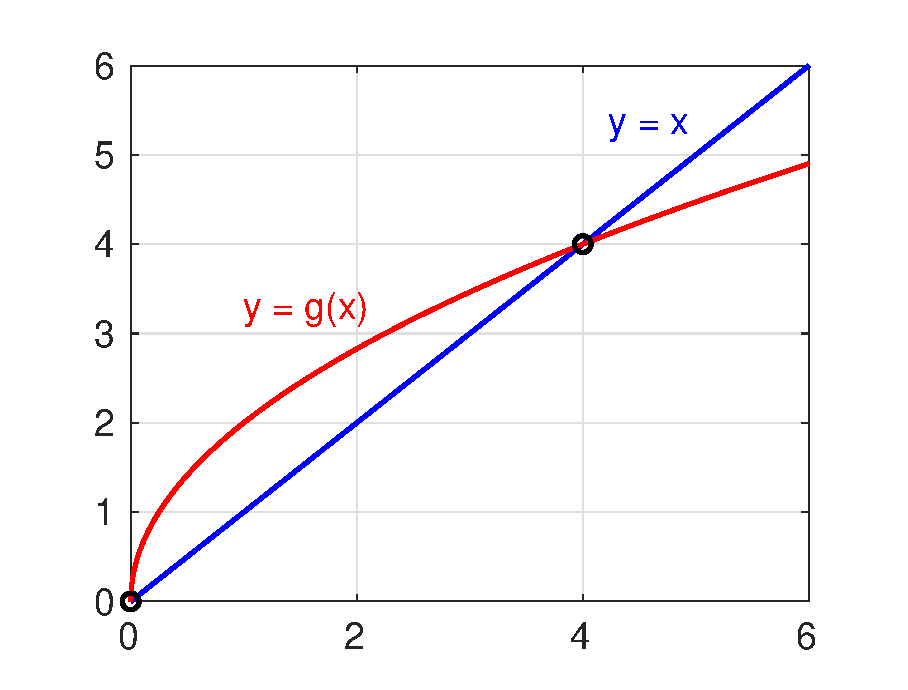
\includegraphics[width=\textwidth]{figures/fixiter}}}%
{I and II}%
{II and III}%
{I and III}%
{I, II and III}%
{3}{}{\mah}

%%%%%%%%%%%%%%%%%%%%%%%%%%%%%%%%%%%%%%%%%%%%%%%%%%%%%%%%%%%%%%%% 
% Multiple-choice questions with three responses.
\section{MC-3}
\qitemMCthree{Consider the matrix
  \begin{gather*}
    A = \begin{bmatrix}
      4 &  -8 &  1 \\
      6 &   5 &  7 \\
      0 & -10 & -3
    \end{bmatrix} 
  \end{gather*}
  whose $LU$ factorization we want to compute using Gaussian
  elimination.  What will the initial pivot element be without
  pivoting, and with partial pivoting?}%
{0 (no pivoting), \quad 6 (partial pivoting)}%
{4 (no pivoting), \quad 0 (partial pivoting)}%
{4 (no pivoting), \quad 6 (partial pivoting)}%
{3}{}{Heath~\cite{heath-1997}, Review Question
  2.36, p.~70}

%%%%%%%%%%%%%%%%%%%%%%%%%%%%%%%%%%%%%%%%%%%%%%%%%%%%%%%%%%%%%%%% 
% Multiple-choice questions with five responses.
\section{MC-5}
\qitemMCfive{Which of the following statements is TRUE?
  \begin{IVlist}
  \item Simpson's rule is exact for linear functions, $f(x) = ax + b$.
  \item Simpson's rule is exact for second-degree polynomials
    (quadratics), $f(x) = ax^2 + bx + c$.
  \item Simpson's rule is exact for fourth-degree polynomials.
  \end{IVlist}}%
{none is true}%
{I}%
{II}%
{I and II}%
{I, II and III}%
{4}{}{\jms, \courseID lecture notes}

%%%%%%%%%%%%%%%%%%%%%%%%%%%%%%%%%%%%%%%%%%%%%%%%%%%%%%%%%%%%%%%% 
% True-false questions.
\section{TF}
\qitemTF{Let $f(x) = x^2 - 2x +1$. The bisection method can be used to
  approximate the root of the function $f(x)$ pictured.
  \begin{center}
    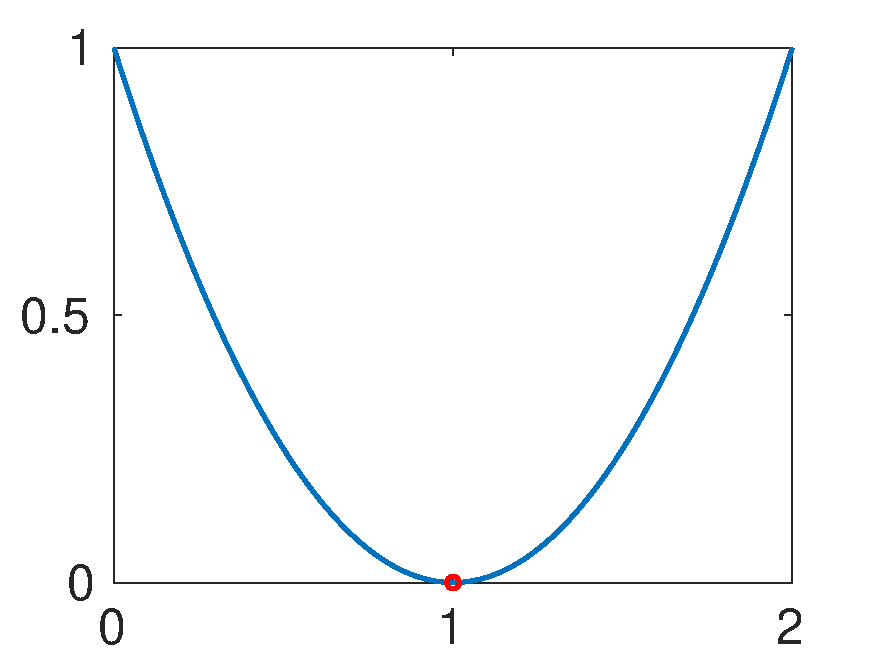
\includegraphics[width=0.45\textwidth]{figures/bisec}
  \end{center}
  \mbox{}}{FALSE}{}{\mah}

\qitemTF{This piecewise polynomial is a quadratic spline:
  \begin{gather*}
    S(x) = \begin{cases}
      0,   & \text{if } -1\leqslant x \leqslant 0 \\
      x^2, & \text{if } 0 \leqslant x \leqslant 1
    \end{cases} 
  \end{gather*}}%
{TRUE}{The piecewise functions are both quadratic, and $S(x)$ and
  $S'(x)$ match at $x=0$.}{\mah}

%%%%%%%%%%%%%%%%%%%%%%%%%%%%%%%%%%%%%%%%%%%%%%%%%%%%%%%%%%%%%%%% 

\end{document}



